\documentclass[a4j,twocolumn]{jsarticle}

\usepackage[top=6.6truemm,bottom=15truemm,left=9truemm,right=9truemm]{geometry}
\usepackage[dvips]{graphicx}
\usepackage{bm}
\usepackage{comment}
\usepackage{amsmath}
\usepackage{amssymb}
\renewcommand{\baselinestretch}{0.85}

\title{Over-smoothing 防止のための層ごとに重み付けするSummarize-GNN}
\author{情報科学専攻~猪口研究室~
47020726~矢嶋 悠太 }
\date{}

\begin{document}
\maketitle

%%%%%%%%%%%%%%%%%%%%%%%%%%%%%%%%%%%%%%%%
\section{はじめに}
\label{sec_introduction}

属性をもつ頂点と辺からなるグラフ構造は、SNSなど実世界の様々なデータを表現できる。
グラフの各頂点を高精度にクラス分類することは、SNSの各ユーザを適切なコミュニティに分類することに対応する。
近年、頂点の高精度なクラス分類のために、グラフを入力として、互いに属性が似ていたり、辺で結ばれている頂点同士が空間上の近い位置にマッピングされるように、各頂点をベクトル表現する、表現学習が注目されている。
頂点のベクトル表現が得られると、既存のクラス分類モデルにそのベクトル表現を入力するだけで、頂点のクラス分類が可能になる。
頂点のクラス分類精度を向上させる、質の高い頂点の表現を学習するために、近年は深層学習を用いた手法であるGraph~Neural~Network~(GNN)\cite{Kipf}が注目されている。

GNNは層数を適切に設定することで高い頂点の分類精度が得られる一方、より多層にすると分類精度が低下する。
GNNを多層化したときに、学習される頂点の表現の質が低下し、分類精度が落ちる現象をOver-smoothingという。
本論文はOver-smoothingの課題を解決することを目的とし、GNNを改良したモデルを提案する。


%%%%%%%%%%%%%%%%%%%%%%%%%%%%%%%%%%%%%%%%
\section{グラフの定義及び問題定義}
\label{sec_definition}

\vspace{-1mm}
グラフを$G=(V,E,X)$とする。ここで$V$は$n$個の頂点集合$\{1,\ldots,n\}$、$E$は頂点$v$から$u$への有向辺$e_{vu}$の集合である。
また、各頂点$v$がもつ属性$\bm{x}_v$は$a$次元のベクトルとし、全頂点の属性の集合を$X=\{ \bm{x}_1, \ldots, \bm{x}_n \}$とする。

頂点のクラス分類について説明する。
全頂点のクラスラベル集合を$Y=\{y_1,\ldots,y_n\}$とする。
グラフ$G$とモデルの学習に用いる教師ラベル集合$Y_{train} \subset Y$を用いて、モデルを学習する。
残りの頂点のラベル集合$Y_{test}=Y \backslash Y_{train}$を用いて、学習済みモデルの分類精度を求める。

本研究では、グラフ$G$を入力とし、全頂点のベクトル表現$H=\{\bm{h}_1, \ldots ,\bm{h}_n\}$を出力することを目的とする。
具体的には、頂点の分類精度を向上させる質の高い$H$を出力するモデルを提案する。


%%%%%%%%%%%%%%%%%%%%%%%%%%%%%%%%%%%%%%%%
\section{近傍内の頂点の属性を集約するGNN}
\label{sec_gnn}

GNNは、$G$と層数$L$を入力とし、頂点$v$の表現$\bm{h}_v$を求める。
\begin{align}
  & \bm{h}_v^l = \text{Conv}(H^{l-1}, N(v)) = \sigma\left( W^l \sum_{u\in N(v)} w_{vu}^l\bm{h}_u^{l-1} \right) \label{eq_gnn1} \\
  & \bm{h}_v   = \bm{h}_v^L \label{eq_gnn2}
\end{align}
頂点$v$自身を含む、有向辺$e_{vu}$により$v$に接続されている頂点の集合$:\{v\} \cup \{u ~|~ e_{vu} \in E\}$を「$v$の1近傍内」と呼ぶ。
また、$\bm{h}_v^0$は属性$\bm{x}_v$、$\sigma(\cdot)$は活性化関数である。
$l-1$から$l$層に進む度、式(\ref{eq_gnn1})の畳み込み$\text{Conv}$により、頂点$v$の潜在表現$\bm{h}_v^{l-1}$を$\bm{h}_v^{l}$に更新する。
各$l$層の$\text{Conv}$では以下を順に実行する。\vspace{-1mm}
\begin{itemize}
  \item[1.] $v$の1近傍内の各頂点$u\in N(v)$の表現を足し合わせる集約\vspace{+1mm}
  \item[2.] 行列$W^l$と活性化関数$\sigma(\cdot)$による線形及び非線形な変換\vspace{-1mm}
\end{itemize}
よって、Convを2回繰り返して得られる表現$\bm{h}_v^2$には、$v$の1近傍内である$u\in N(v)$の、更に1近傍内である$u' \in N(u)$の属性$\bm{x}_{u'}$が集約される。
つまり、$\bm{h}_v^2$には2近傍内の頂点$u' \in N(v,2)$の属性$\bm{x}_{u'}$が集約される。

式(\ref{eq_gnn2})より、GNNは$\text{Conv}$を層数$L$回繰り返して得られる、$L$近傍内の頂点の属性が集約された$\bm{h}_v^L$を$\bm{h}_v$として出力する。



%%%%%%%%%%%%%%%%%%%%%%%%%%%%%%%%%%%%%%%%
\section{GNNの課題:Over-smoothingへの一考察}
\label{sec_oversmoothing}

GNNは層数$L$を適切な層数$L_v^*$に設定することで、質の高い表現を得ることができ、近年最高峰の分類精度を達成している。
一方、GNNの層数$L$を$L_v^*$より大きくする程、表現$\bm{h}_v(=\bm{h}_v^L)$の質が低下し、その後のクラス分類精度も低下する現象をOver-smoothingと呼ぶ。
適切な層数$L_v^*$のGNNが質の高い表現を得て、より多層$L(\le L_v^*)$のGNNが質の低い表現を得る理由について、本資料では、教師ラベル$Y_{train}$を用いることなく独自の観点から考察していく。

考察のため、図の例を

%%%%%%%%%%%%%%%%%%%%%%%%%%%%%%%%%%%%%%%%
\section{提案手法}
\label{sec_proposal}

\vspace{-2mm}
JKNetが用いるAD~Attentionに対し、我々は$\bm{f}_i^l$と$\bm{b}_i^l$間の類似度を求めるDot-product Attention~(DP Attention)\cite{Vaswani}を用いて頂点$v_i$から$N_{v_i}^l$への注目度$e_{v_i}^l$を求める。

\vspace{-2mm}
\begin{equation}
  e_{v_i}^l = dp(\bm{f}_i^l, \bm{b}_i^l) = \frac{\bm{f}_i^l~ \cdot ~\bm{b}_i^l}{\sqrt{d'}} \label{eq_DP_Attention}
\end{equation}
\vspace{-4mm}


JKNetと本論文で用いるADとDP Attentionの機構の違いが注目度$e_{v_i}^l$に与える影響について説明するために、図\ref{fig_alpha}の具体例を用いて説明する。
また、クラス1に属する頂点らの$j$番目の属性値は同じ正規分布$N(\mu_1^j, \sigma_1^j)$に従い、異なるクラス2に属する頂点らの属性値は$N(\mu_2^j, \sigma_2^j)$に従うと仮定する。

\vspace{-2mm}
\begin{equation}
  x_i^j \sim
      \begin{cases}
          N(\mu_1^j, \sigma_1^j)    &   \text{$v_i$がクラス1に属するとき} \nonumber \\
          N(\mu_2^j, \sigma_2^j)    &   \text{$v_i$がクラス2に属するとき} \nonumber
      \end{cases}
\end{equation}

\vspace{-1mm}
\noindent
図\ref{fig_alpha}のグラフ$G=(V,E,X)$のみを入力として、$v_{16}$の$N_{v_{16}}^l$への注目度$e_{v_{16}}^l$を$L=7$層のAttention~GNNで学習することを考える。
\ref{sec_attention}節で述べたように、$\bm{b}_{16}^l$には$N_{v_{16}}^L$の属性が集約される。
$L=7$のため、$N_{v_{16}}^7$は図\ref{fig_alpha}紫の実線で示されるように、クラス1と2に属するすべての頂点で構成される。
よって図\ref{fig_alpha}下の紫の棒グラフで示されるベクトル$\bm{b}_{16}^4$と$\bm{b}_{16}^6$には、$N(\mu_1^j, \sigma_1^j)$に従う属性と$N(\mu_2^j, \sigma_2^j)$に従う属性が混合される。

一方、$\bm{f}_{16}^l$には$N_{v_{16}}^l$の属性が集約される。
$l=4$のとき、$N_{v_{16}}^4$は図\ref{fig_alpha}左の青の破線のように、$v_{16}$と同じクラス2に属する頂点のみで構成される。
よって図\ref{fig_alpha}左下の青の棒グラフの$\bm{f}_{16}^4$は、$N(\mu_2^j, \sigma_2^j)$に従う属性のみからなる。
$l=6$のとき、$N_{v_{16}}^6$は図\ref{fig_alpha}右の紫の破線のように、クラス1と2の両方に属する頂点で構成される。よって図\ref{fig_alpha}右下の紫の棒グラフの$\bm{f}_{16}^6$には、$N(\mu_1^j, \sigma_1^j)$に従う属性と$N(\mu_2^j, \sigma_2^j)$に従う属性が混合される。

$v_{16}$は半径$l$が1から4までの$N_{v_{16}}^l$に注目すると望ましい。つまり注目度$e_{v_{16}}^l$が高いことが望ましい$l=4$(図\ref{fig_alpha}左)のとき、$\bm{f}_{16}^4$と$\bm{b}_{16}^4$間の類似度は低い。
一方、$e_{v_{16}}^l$が低いことが望ましい$l=6$(図\ref{fig_alpha}右)のとき、$\bm{f}_{16}^6$と$\bm{b}_{16}^6$間の類似度は高い。

\begin{figure}[b]
  \begin{minipage}{0.49\hsize}
   \begin{center}
    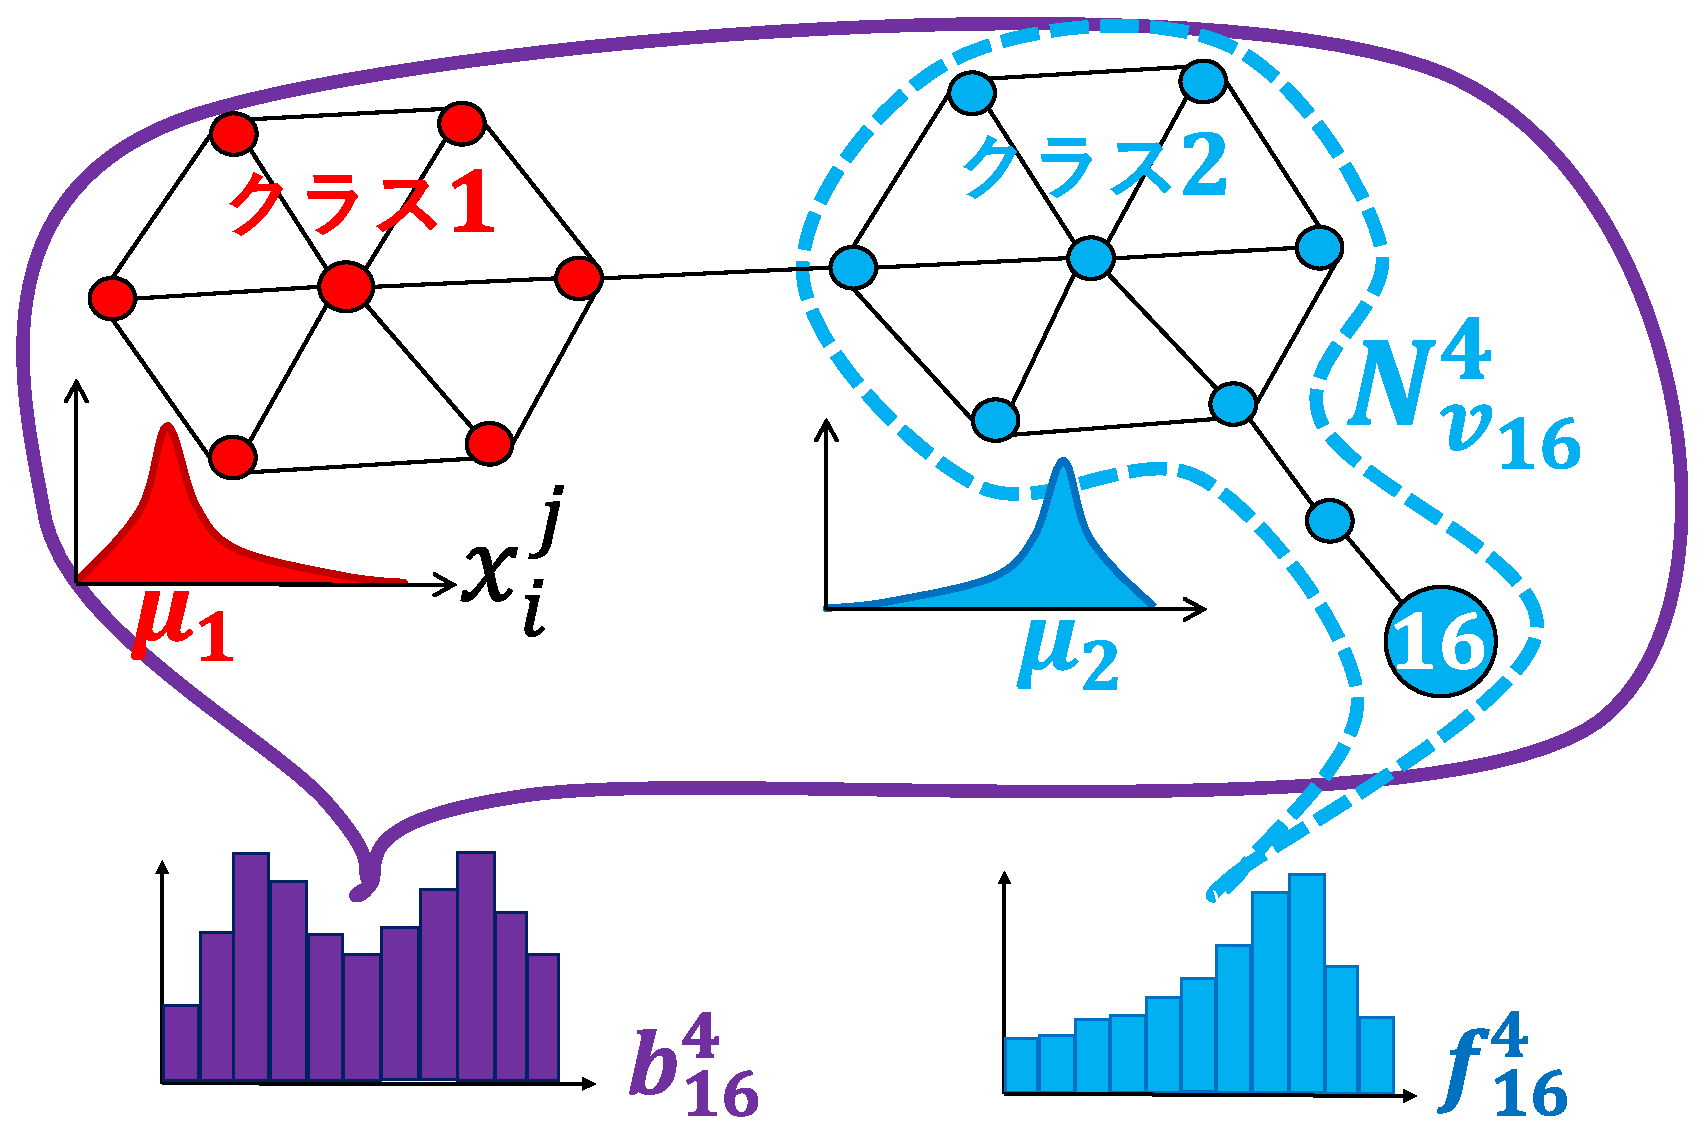
\includegraphics[height=52mm,width=46mm]{alpha_l4.eps}
   \end{center}
  \end{minipage}
  \begin{minipage}{0.49\hsize}
  \begin{center}
   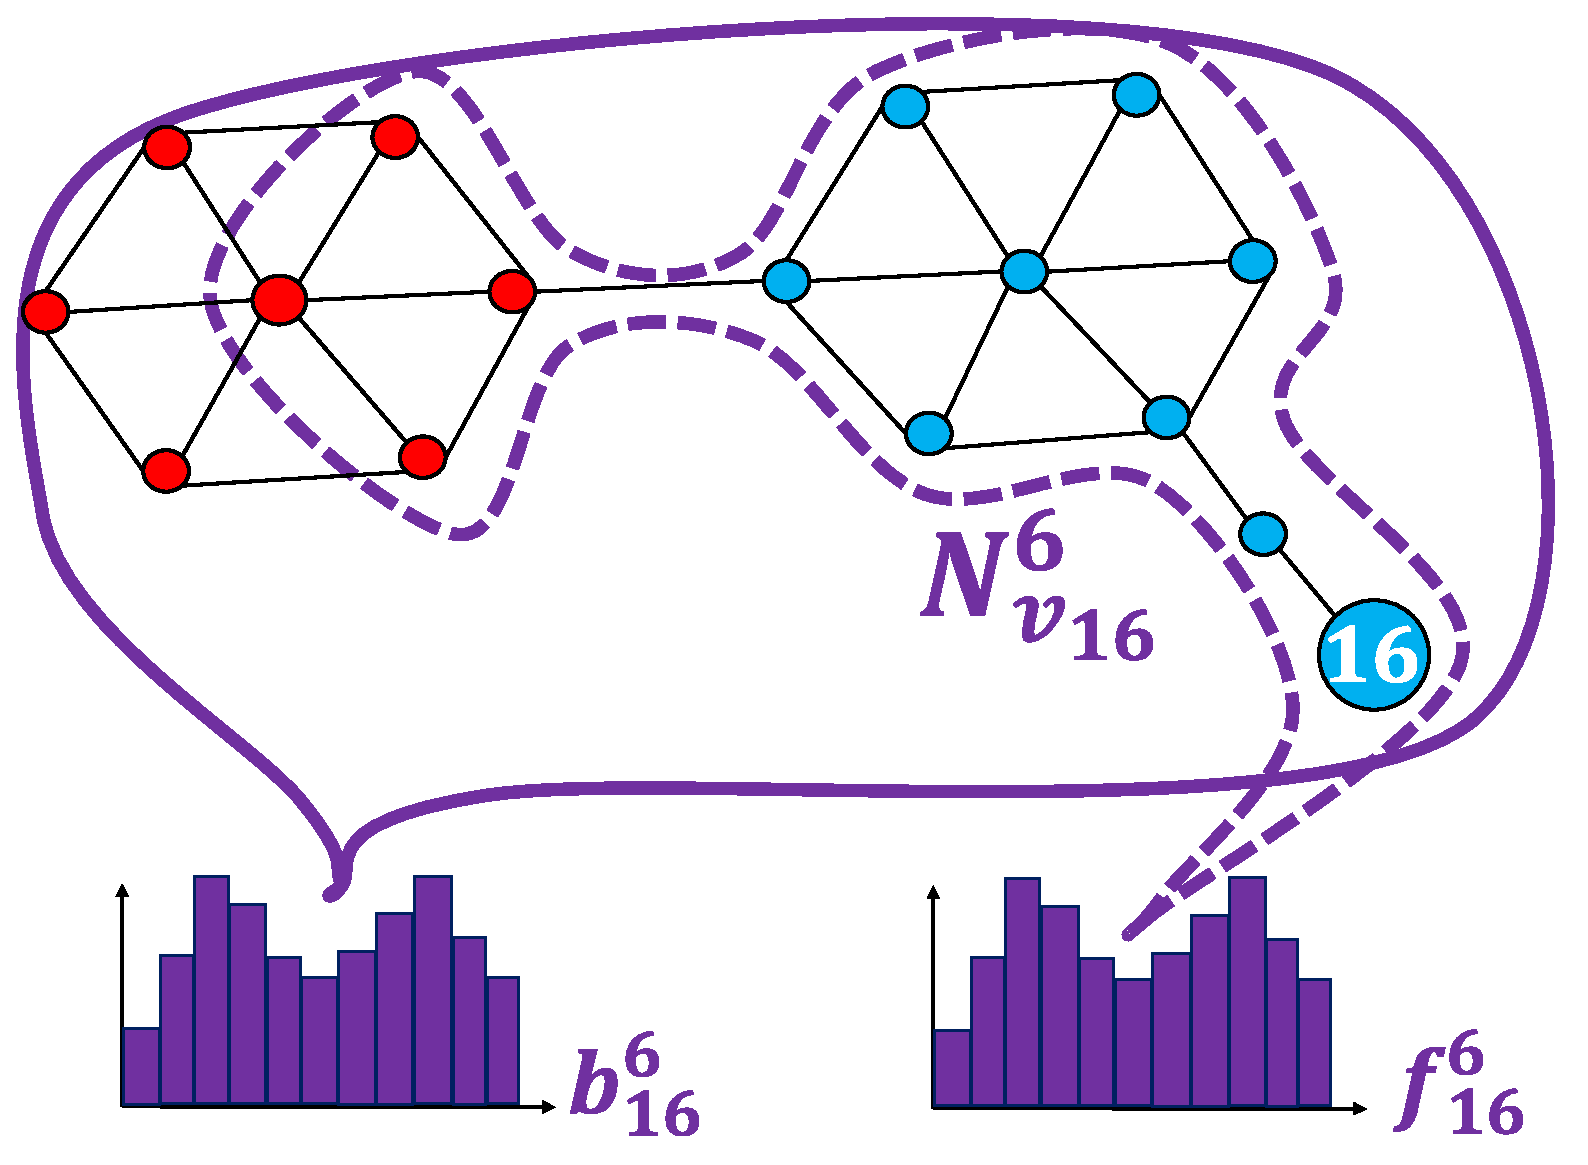
\includegraphics[height=52mm,width=46mm]{alpha_l6.eps}
  \end{center}
  \end{minipage}
\vspace{-1mm}
\caption{$l=4,6$のときの$\bm{f}_{16}^l$と$\bm{b}_{16}^l$に属性が集約される様子}
\label{fig_alpha}
\end{figure}

この、$\bm{f}_i^l$と$\bm{b}_i^l$間の類似度の大小が、望ましい注目度$e_{v_i}^l$を求めるヒントになることに着想を得て、本論文では$\bm{f}_i^l$と$\bm{b}_i^l$間の類似度を求める、式(\ref{eq_DP_Attention})のDP Attentionを用いる。
更に、ADとDPを混合した機構であるMX Attention\cite{Kim}も用いる。

\vspace{-1mm}
\begin{equation}
  e_{v_i}^l = mx(\bm{f}_i^l, \bm{b}_i^l) = ad(\bm{f}_i^l, \bm{b}_i^l) \times \sigma(dp(\bm{f}_i^l, \bm{b}_i^l)) \label{eq_MX_Attention}
\end{equation}
\vspace{-5mm}

\noindent
ただし、$\sigma(\cdot)$はシグモイド関数である。

式(\ref{eq_DP_Attention})のDPまたは式(\ref{eq_MX_Attention})のMX~Attentionを用いた我々のAttention~GNNは、式(\ref{eq_JKNet})のAD Attentionのみ用いるJKNetより、頂点ごとに理想的な半径の$N_{v_i}^l$からの属性の集約が可能であり、Over-smoothingの防止につながることが期待できる。

%%%%%%%%%%%%%%%%%%%%%%%%%%%%%%%%%%%%%%%%
\section{評価実験}
\label{sec_experiment}

\vspace{-2mm}
我々のDPまたはMX~Attention~GNNとJKNet\cite{Xu1}のAD~Attention~GNNを、どちらがOver-smoothingの防止性能が高いか、という観点から比較する。
比較のため、各GNNによって頂点の表現学習とクラス分類をする。
データセットは、タンパク質とその相互作用からなるPPI、電子掲示板に投稿するユーザとその関係からなるRedditの2つを用いる。

GNNにより学習される各頂点の表現$\bm{h}_i$を入力として、線形変換とsoftmax関数により、クラスラベルの予測$\bm{\hat{y}}_i$を得る。訓練時は教師信号として与えられた一部のクラスラベルと予測$\bm{\hat{y}}_i$の誤差を求め、誤差逆伝搬法でGNNのパラメータを学習する。
テスト時はGNNが正しく予測できたクラスラベルの割合$Acc$を求め、$Acc$の高さをGNNのクラス分類の性能とする。

図\ref{fig_accuracy}は、横軸を各GNNの層数$L$、縦軸を$L$層のGNNでクラス分類したときの$Acc$として表す。
我々のDPまたはMX~Attention~GNNでクラス分類したときの$Acc$を赤色で、JKNetのAD~Attention~GNNでクラス分類したときの$Acc$を青色の折れ線で表している。
多層にしても、つまり横軸方向に進んでも、$Acc$を低下させずに維持できるAttention~GNNほど、Over-smoothingの防止性能が高いといえる。

PPIとRedditデータセット共に、両Attention~GNNは、多層にしても$Acc$を維持できる点では共通するが、DPまたはMX~Attention~GNNの方がより高い$Acc$を維持できている。

\begin{figure}[b]
  \centering
  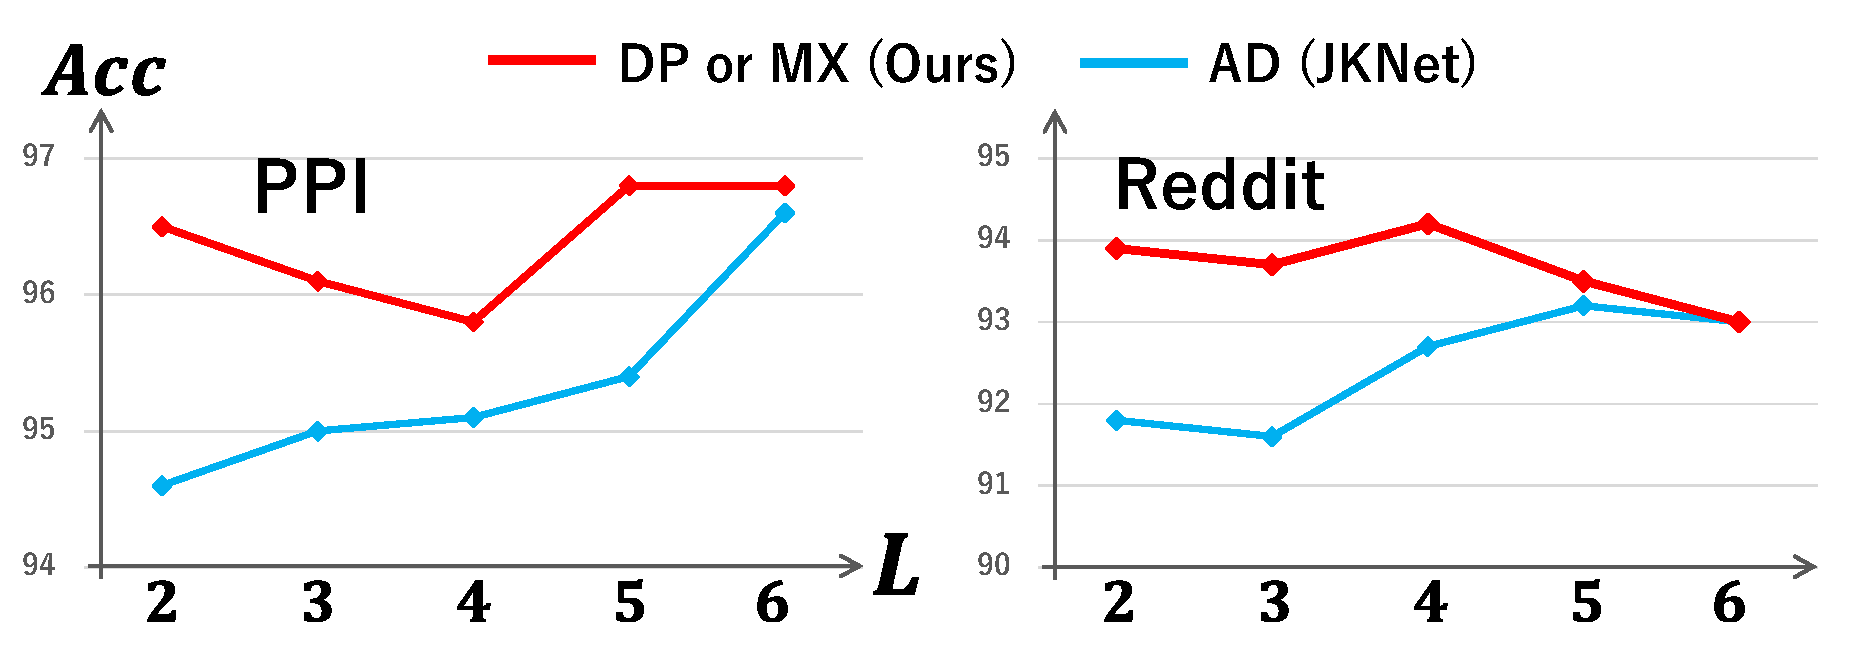
\includegraphics[height=4.2cm,width=9.4cm]{acc.eps}
  \vspace{-7mm}
  \caption{各GNNの層数$L$に対するクラス分類の$Acc$}
  \label{fig_accuracy}
\end{figure}

%%%%%%%%%%%%%%%%%%%%%%%%%%%%%%%%%%%%%%%%
\section{まとめと今後の展望}

\vspace{-2mm}
Over-smoothingの防止のため、頂点ごとに理想的な半径の$N_{v_i}^l$から属性を集約することを目的として、DP及びMX~Attention~GNNを提案した。
実データセットを用いた評価実験によって、同じ目的のJKNetが提案したAD~Attention~GNNよりもOver-smoothingの防止性能が高いことが示された。
今後は、他のデータセットでも同様の実験を行う予定である。

%%%%%%%%%%%%%%%%%%%%%%%%%%%%%%%%%%%%%%%%

\bibliographystyle{jplain}
\renewcommand{\bibname}{参考文献}
\begin{thebibliography}{1}
\addcontentsline{toc}{chapter}{参考文献}
\markboth{参考文献}{参考文献}
\vspace{-2mm}

\bibitem{Kipf}
T. N. Kipf, M. Welling.:
Semi-supervised classification with graph convolutional networks,
{\it arXiv Preprint}, arXiv:1609.02907 (2016).
\vspace{-0.3mm}

\bibitem{Xu1}
K. Xu, et al.:
Representation learning on graphs with jumping knowledge networks,
{\it ICML}, pp.~5453--5462. PMLR (2018).
\vspace{-0.3mm}

\bibitem{Vaswani}
A. Vaswani, et al.:
Attention is all you need,
{\it NIPS}, pp.~5998--6008 (2017).
\vspace{-0.3mm}

\bibitem{Hochreiter}
S. Hochreiter, J. Schmidhuber.:
Long short-term memory,
{\it Neural Computation}, 9.8: pp.~1735--1780 (1997).
\vspace{-0.3mm}

\bibitem{Kim}
D. Kim, A. H. Oh.:
How to find your friendly neighborhood: Graph attention design with self-supervision,
{\it ICLR}, (2020).
\vspace{-0.3mm}

\end{thebibliography}
\end{document}